\section{Автоматизация среднего образования с помощью ostis-систем}
\label{sec_automation_secondary_education}

\begin{SCn}
	
	\bigskip
	
	\begin{scnrelfromlist}{ключевое понятие}
		\scnitem{интеллектуальная обучающая система}
		\scnitem{семантический электронный учебник}
		\scnitem{компьютерные средства обучения}
	\end{scnrelfromlist}
	
	\bigskip
	
	\begin{scnrelfromlist}{ключевое знание}
		\scnitem{...}
	\end{scnrelfromlist}
	
	\bigskip
	
	\begin{scnrelfromlist}{библиографическая ссылка}
		\scnitem{\scncite{Eliseeva2013}}
		\scnitem{\scncite{...}}
		\scnitem{\scncite{...}}
		\scnitem{\scncite{...}}
		\scnitem{\scncite{...}}
		\scnitem{\scncite{...}}
	\end{scnrelfromlist}
	
\end{SCn}

\textit{Интеллектуальные компьютерные системы} создаются для того, чтобы на них можно было перенаправить часть человеческой деятельности. По мере развития методов и средств деятельности человека интеллектуальные системы самосовершенствуются, обучают самих себя на основе накопленного опыта и используя огромную базу знаний, которые являются доступными для компьютеров в кратчайшие моменты времени. Поскольку \textit{интеллектуальная компьютерная система} может довольно быстро обучить саму себя, то она может обучить и других. Если изначально, человек составляет алгоритмы, программы для обучения компьютерной системы, то затем он может получать и использовать знания, полученные интеллектуальной системой из информационной базы данных. Следовательно, \textit{интеллектуальная компьютерная система} способна сама обучать человека, то есть стать помощником в такой важной сфере человеческой деятельности, как образование. Здесь особую роль играют семантические интеллектуальные системы, которые используют смысловые взаимосвязи, то есть делают то же, что и человек, но в миллионы раз быстрее. Семантические интеллектуальные системы позволяют, с одной стороны, ускорить процесс получения знаний на основе получения моментального доступа к огромному информационному полю, а с другой стороны, интеллектуальные системы должны помочь выбрать оптимальный путь обучения, путь по которому в наиболее короткие сроки будут получены полные знания.

Школьное образование является важным этапом, который формирует все дальнейшее развитие образования индивидуума. Если школьное образование соответствует слишком низкому уровню, то никакие последующие этапы этого не исправят. Невозможно из неграмотного, неподготовленного человека получить хорошего инженера. Если нет основы знаний, то нельзя построить и базис знаний более высокого уровня. Поэтому рассмотрение вопроса образования мы начнем со школьного образования, тем более многие проблемы и вопросы, возникающие в сфере образования более высоких ступеней совпадают с проблемами школьного образования, либо являются их следствием.

Существует много интересного в различных сферах: истории, географии и так далее.  Очень интересно смотреть фильмы, читать книги и расширять свой кругозор. Можно участвовать в различных викторинах, квестах, разгадывать кроссворды. Но цель образования не просто расширить кругозор знаний ученика, а помочь ему определиться с выбором сферы деятельности согласно его способностям и потребностям общества.

При рассмотрении вопросов и способов достижения этой цели необходимо исходить из определения характеристик продукта, который надо получить в итоге. К обобществленным характеристикам качества и количества знаний выпускников различных учебных заведений можно отнести:
\begin{textitemize}
	\item компетенции --- комбинация знаний, навыков и опыта, необходимых для качественного выполнения поставленных задач;
	\item широта знаний --- набор знаний из различных областей, способных дополнять друг друга и формировать единую картину окружающего мира;
	\item глубина знаний --- характеристика, показывающая в каком объеме и на каком уровне сложности человек обладает знаниями по тому или иному вопросу или явлению.
\end{textitemize}

Но чтобы правильно выстроить процесс образования той или иной ступени необходимо конкретно очертить набор знаний (явлений, законов, формул и тому подобное), которыми должен обладать выпускник по тому или иному конкретному учебному предмету.
\begin{textitemize}
	\item ступень образования --- самостоятельный завершенный этап обучения и воспитания системы образования;
	\item учебный предмет --- система знаний, умений и навыков, отобранных их определенной отрасли человеческой деятельности.
\end{textitemize}

Также необходимо чтобы учебные программы каждого года обучения по предметам дополняли и расширяли, а не дублировали, знания, полученные в предыдущие годы обучения. Программы обучения по предметам и сам процесс обучения должны соответствовать некоторым принципам (правилам, требованиям), которые будут рассмотрены далее.  

\textbf{При составлении учебных программ} надо учитывать взаимосвязь между различными учебными дисциплинами. Знания, полученные по одним учебным дисциплинам, используются при изучении других дисциплин. Например: при изучении по физике тем раздела «простые механизмы» вычисление момента силы требует определения величин проекций, а для этого необходимы знания о соотношениях между величинами углов и сторон в прямоугольных треугольниках, знания простейших тригонометрических функций. При изучении в механике векторных характеристик движения и взаимодействия тел требуются знания понятия «вектор» и простейших операций с векторами, а также знания соотношении углов и сторон в прямоугольных прямоугольниках для нахождения проекций векторов на заданные оси. Эти знания требуются для рассмотрения всех видов сил и нахождения их равнодействующих. На основе знаний, полученных при изучении различных разделов физики, можно объяснять различные темы, изучаемые в других дисциплинах: химии, географии и другие.

В тоже время \textbf{использование знаний}, полученных в других предметах, \textbf{позволяет закрепить эти знания}. Например, использование знаний о тригонометрических функциях, проекциях, векторах при решении физических задач позволяет закрепить, углубить и обосновать эти знания, полученные из математики. Применение этих знаний в физике \textbf{позволяет сократить время}, отведенное для изучения и освоения тем в геометрии. 

Также \textbf{рассмотрение нового материала}, его освоение в рамках решения задач, \textbf{должно способствовать повторению ранее пройденного материала} по этому и другим, смежным предметам. Если на начальном этапе даются задачи непосредственно по этому материалу (на формулу). Но для действительного знания темы нужно уметь решать задачи, при решении которых надо использовать наряду с материалом изучаемой темы знания, полученные ранее при изучении других тем в рамках этого или других предметов. Это позволяет улучшить усвоение материала, обеспечить практически постоянную повторяемость материала, постепенное усложнение решаемых задач, учесть взаимосвязь различных явлений, выйти на новый уровень знания и сократить время, затрачиваемое на простое, банальное повторение материала. Также это дает возможность исключить дублирование при рассмотрении материала в старших классах. 

\textbf{Рассмотрение явлений и законов}, изучаемых в различных разделах учебных предметов (независимо от времени изучения) на каждом этапе должно быть \textbf{полным} и не может иметь незаконченный вид из-за того, что школьники не обладают какими-либо предварительными данными. Также необходимо учитывать логичность и связываемость получаемых знаний, чтобы знания не превращались в набор отрывочных сведений и определений, требующих банального запоминания. Логическое осмысливание материала, построение связей этого материала с имеющимися знаниями и окружающей действительностью являются главными составляющими индивидуального опыта. Знания выступают в форме понятий и отношений между ними, а также производных от них суждений и умозаключений обучающегося. Именно такие знания в виде навыков и умений лучше хранятся в памяти обучаемого.

\textbf{Взаимодополнение} одних предметов другими возможно, если изучение различных дисциплин в школьном курсе будет тесно увязано, как по изучаемым темам, так по времени прохождения учебного материала в том или ином курсе. На данный момент, то что ученики 8-х классов не проходят до этого времени по геометрии тригонометрических функций, не дает возможности полностью рассмотреть такие темы по физике, как рычаги, силы и взаимодействие тел, преломление света и др. Поэтому необходимо корректировать программы изучения дисциплин для своевременного использования знаний при изучении других дисциплин. 

Надо также рассмотреть вопрос о наполнении содержания учебного материала по каждой теме в каждой отдельной дисциплине. Необходимо учитывать, что \textbf{существуют определенные ограничения} как по сложности, так и по объему нового материала, который \textbf{может воспринять школьник} в отведенное для этого время, чтобы избежать перегрузок, которые могут негативно отразиться на его здоровье. Наиболее эффективно осваиваются темы, которые отображены в окружающем нас физическом и информационном пространстве в силу их жизненной востребованности. Темы, которые не находят отображения в окружении и не требуются для получения необходимых жизненных навыков должны быть выведены из обязательного программного школьного материала и даваться в наиболее компактном виде на уровне ознакомления. Более расширенное рассмотрение этих тем должно быть выведено из программного школьного материала и проводиться в рамках факультативного и дополнительного образования. Таким образом, изучаемые дисциплины должны быть освобождены от излишнего сопутствующего материала, который увеличивает количество информации, нагрузку на память школьника, но не несет никакой дополнительной информации, помогающей понимать суть явлений и изучать их, а соответственно просто отнимает учебное время. Это касается каждого изучаемого предмета, каждой темы на определенных этапах их изучения. Формирование содержания учебной дисциплины в рамках программы должно исходить не из того, что один или два урока в неделю выделяется для изучения предмета, а из количества и содержания учебного материала, который \textbf{необходимо} освоить в текущем учебном году.  Соответственно, на некоторые предметы может быть выделено 10 учебных часов, а на другие в 2--20 раз больше. Это особенно актуально стало в данное время в связи с тем, что стремительно увеличивается количество информации и появляются новые предметные области, освоение которых необходимо в современной жизни.

Удовлетворение программ обучения и самого процесса обучения этим принципам способствует тому, что различные дисциплины будут формировать всесторонние знания об окружающем мире.

При рассмотрении вопросов, связанных с образованием, нельзя обойти вниманием аспект, связанный с индивидуальностью каждого обучаемого. У каждого школьника есть способности и предрасположенности к тем или другим предметам. Учет этих факторов обеспечивает максимально возможное раскрытие творческого потенциала каждого человека. Развитию этих способностей и подготовке школьников к выбору профессиональной деятельности в дальнейшей жизни должно служить дополнительное и факультативное образование. На уровне такого образования можно осуществить более персонализированный подход к каждому ученику, при котором становится возможным полное раскрытие творческого потенциала каждого. При этом надо давать по выбранным дисциплинам более обширные и глубокие знания. Получение дополнительного образования должно учитываться при расчетах временной и физическо-умственной нагрузки учащихся.

Кроме того вопросы организации среднего образования необходимо тесно увязывать с организацией образования на последующих ступенях. Фундамент знаний, их база, сформированные в школе являются той стартовой точкой, с которой начинается следующий этап в жизни обучающегося. Рамки этих знаний четко обозначены школьной программой, следовательно на основе этого становится понятным, какие разделы и на каком уровне должны изучаться далее для освоения той или иной специальности.

К сожалению, надо отметить, что последние годы наблюдается спад уровня школьного образования выпускников. Введение новых учебных программ не позволяет исправить данную ситуацию. Существуют различные субъективные и объективные причины, приводящие к этой ситуации. Это и резкое увеличение количества информации по различным разделам, вызванное развитием науки и увеличением доступности информации. Это инертность изменчивости школьных программ. Одной из причин является и то, что программы и учебники по разным курсам составляются разными людьми, специализирующимися в отдельных областях знаний. Эти люди не видят общей картины формирующихся знаний, пытаются наполнить свой предмет как можно более глубокими новыми данными и определениями, увеличить количество часов, отведенных для изучения предмета в школе. Иногда такое увеличение материала приводит к тому, что школьная программа по некоторым разделам предмета практически не отличается от программ высших учебных заведений. По мнению этих авторов это приводит к заинтересованности в их предмете, улучшению качества знаний по предмету. На самом деле, это приводит только к тому, что школьникам приходится запоминать намного больше информации (иногда не связанной), что приводит к перегрузке и запутыванию учащихся.

Никакая группа специалистов не сможет до конца учесть и просчитать все вопросы, связанные с образованием, так как эти проблемы являются многонаправленными и многоуровневыми. Традиционная образовательная система не может обеспечить выпускникам своевременный должный уровень знаний. Образование является той сферой деятельности, которой предстоит особенно серьезная перестройка. Для поддержания высокого уровня востребованности на рынке труда учащиеся должны высокими темпами обновлять необходимые знания, объем которых удваивается в среднем каждые полтора года, что требует постоянной переподготовки. Решить проблему можно с помощью создания интеллектуальных компьютерных систем образования, базирующихся на очень объемных базах знаний. Такие системы должны позволить исправить ошибки, допускаемые в подходах к освоению знаний, более быстро и эффективно учитывать изменения в требованиях к компетенциям выпускников, которые появляются с развитием научных и технических знаний и материально-технической базы общества. Цифровые технологии позволят создать систему образования, которая будет более эффективной и сбалансированной. 

Что же должна уметь интеллектуальная система и какой базой знаний она должна обладать?

База знаний должна быть многоуровневой.

В интеллектуальной системе должна быть сформирована \textit{база знаний}, охватывающая все знания, которыми при окончании школы должен обладать выпускник. В противном случае будет отсутствовать глубокая конвергенция между деятельностью по подготовке учеников и тем багажом знаний, которым они должны обладать по окончании школы. Эта часть общей базы знаний должна охватывать все предметы школьной программы, но только в объеме, достаточном для понимания и усвоения информации по каждому предмету. Также в \textit{базе знаний} должна быть учтена проблема объема информации с учетом сложности материала, который может быть освоен в тот или иной период обучения. На основании этих знаний интеллектуальная система должна сформировать программу обучения, распределить в какой период обучения изучаются конкретные разделы различных предметов и на каком уровне формируются знания в этот период. При этом интеллектуальная система должна учитывать, какими знаниями обладает обучаемый, когда приступает к изучению новой темы. К этому моменту школьник должен знать все необходимые предпосылки, обладать знаниями по этому и другим предметам, необходимыми для изучения темы. В результате должно быть сформировано сбалансированное распределение всего изучаемого материала из различных предметов по времени. Так как объем изучаемого материала с учетом сложности и время обучения имеют конечное значение, то интеллектуальная система должна ограничить количество материалов, даваемых на обучение в каждый период времени, и отрезать материалы, которые только увеличивают количество запоминаемых данных, но не несут никакой дополнительной информации, необходимой для понимания и освоения основных законов и явлений. В результате должна быть создана модель предметной области по каждой дисциплине с учетом междисциплинарных связей. В этой связи очень важно обеспечить технологические средства "перехода"{} границ между учебными материалами различных учебных дисциплин. Модель предметной области играет главную роль, поскольку она используется для решения задач структуризации и систематизации учебного материала, реализации навигационно-поисковых алгоритмов по учебному материалу и реализации адаптивного управления обучением и др. В идеале, обучаемый должен иметь возможность при решении целого ряда задач работать с учебным материалом не в масштабе отдельной учебной дисциплины, а в масштабе всех дисциплин, касающихся изучаемого вопроса. Необходимо упомянуть и о логической организации учебного материала в рамках специальности, которая позволяет выявить связи учебных дисциплин, определенных тем этих учебных дисциплин, их составляющих фрагментов (теорем, определений понятий и др.) с другими учебными дисциплинами, темами, фрагментами учебного материала последующими и предыдущими. Появляется возможность определить более рациональную последовательность изучения учебного материала. Система управления знаниями, находящаяся в \textit{базе знаний}, должна также обеспечивать сбор и систематическую организацию, анализ данных и знаний из различных источников, пополнение \textit{базы знаний} изнутри самой системы. 

Кроме того должна быть создана интеллектуальная подсистема с открытой самодополняющейся \textit{базой знаний}, которая будет расти со временем по мере прохождения тем по различным предметам. Образовательный подход на основе постепенного наполнения обучающегося знаниями и умениями через постепенное их представление в рамках набора дисциплин остается актуальным. На каждом этапе обучения ученику должен быть доступен уровень знаний в базе знаний, соответствующий пройденному им материалу. обучения на основе этих оценок, то есть интеллектуальная система должна сама состоять из целого ряда подсистем, содержащих базы знаний, семантически коррелированные между собой.

Индивидуальная деятельность учащихся является важной составляющей образования, которая формирует навыки обучаемого, способствует наиболее эффективному усвоению знаний, определяет его наклонности и способствует их развитию. Индивидуальная деятельность присутствует при различных способах изучения информации: обучение по обязательной программе, дополнительное факультативное индивидуальное обучение. При дополнительных видах обучения может использоваться информация, не входящая в обязательную школьную программу. Такая более широкая информация должна быть доступна школьникам, но находиться она должна в общей базе знаний и использоваться для дополнительного, факультативного или самостоятельного образования. Освоение этой информации должно происходить вне основного школьного обучения, как по временным, так и по информационно-программным компонентам и способствовать развитию индивидуальных способностей обучающихся.

При любом виде обучения  с участием интеллектуальных обучающих систем учащему необходим помощник --- интеллектуальный персональный ассистент, который  поможет наладить общение с интеллектуальной системой и сделать ее использование наиболее эффективным. Персональный ассистент каждого участника-пользователя включается в систему, чтобы уже на этапе первого взаимодействия пользователя с интеллектуальным интерфейсом обеспечить как безопасность системы, так и комфорт работы пользователя. Адаптивный подход к проектированию пользовательского интерфейса в обучающих системах является одним из перспективных направлений развития указанного класса систем. Данный подход предусматривает создание гибкой структуры диалога системы с пользователем в соответствии с рядом индивидуальных характеристик пользователя: подготовленность к работе с системой, характеристик взаимодействия с системой, интерфейсных предпочтений, индивидуальных психологических характеристик.

Поскольку, развитие образовательной системы предполагается организовывать на базе
общей \textit{ostis-системы}, то естественно необходимо использовать и общие подходы при построении отдельных подсистем. Разрабатываемые общие модели интерфейса \textit{метасистемы OSTIS} необходимо адаптировать для образовательной OSTIS системы. Это позволит значительно снизить материальные и временные затраты на построение интерфейса системы.

Наряду с задачей создания персонального пользовательского интерфейса, у персонального ассистента существует много других задач. Он формирует спектр информации об обучаемом. Определяет его наклонности и способности в той или иной области знаний.

Персональный ассистент при рассмотрении отдельных изучаемых тем помогает сформировать вариант навигации по семантическим связям, когда обучаемый либо система формирует некоторый путь, раскрывает признак, переходит на следующий признак и так дальше по учебному материалу; предлагает задачи на законы из изучаемого материала, на следующем этапе --- задачи, в которых наряду с этим используется материал из ранее пройденных тем, в том числе и из других предметов, далее предлагаются задачи еще более сложного уровня. 

Кроме того персональный ассистент должен сформировать систему оценки результатов на каждом этапе обучения. Это постоянная ненавязчивая диагностика состояния обучаемого и корректировка его модели обучения на основе анализа результатов контроля. Она формируется, с одной стороны, на основе информации о том, сколько времени потратил ученик на изучение темы, задачи какой сложности смог решить и так далее.

С другой стороны, персональный ассистент должен сформировать "разумную"{} вопросно-ответную систему по указанному материалу (то есть систему, способную находить ответы на достаточно большое количество вопросов, касающихся смысла, семантики соответствующего материала).

Корректировка процесса обучения должна происходить на основе этих оценок, формируя набор необходимой информации для следующего уровня, то есть интеллектуальная образовательная система должна сама состоять из целого ряда подсистем, содержащих базы знаний, семантически коррелированные между собой.
Специализированные базы данных и знаний, электронные учебники, в том числе подготовленные с использованием средств гипермедиа и мультимедиа, а также сетевые источники на основе средств Интернет. Таким образом, постоянно повышаются требования к эффективности и практикоориентированности обучающих систем, что приводит к неизбежному осознанию актуальности проблемы разработки таких компьютерных обучающих систем, в которых должна обеспечиваться:
\begin{enumerate}
	\item обработка больших объемов сложноструктурированной информации различного типа;
	\item гибкость и легкая модифицируемость системы;
	\item интеграция различных моделей и механизмов решения задач;
	\item поддержка различных моделей обучения и управления взаимодействием с пользователем;
	\item интеграция различных программных систем в составе одной системы и осуществление управления их функционированием и взаимодействием;
	\item широкое использование средств мультимедиа;
	\item работа в реальном масштабе времени.
\end{enumerate}

Сформулировать основные требования, предъявляемые к интеллектуальным обучающим системам, следующим образом:

\begin{textitemize}
	\item \textbf{Универсальность}. Наличие средств представления и обработки учебных и учебно-методических знаний, ориентированных на любую предметную область.
	\item \textbf{Адаптивность}. Наличие средств формирования модели обучаемого и средств адаптации образовательного процесса к обучаемому.
	\item \textbf{Гибкость}. Наличие средств, позволяющих реализовывать различные модели обучения, а также поддерживающих различные формы обучения.
	\item \textbf{Расширяемость}. Возможность модифицировать существующие свойства системы и добавлять новые свойства без нарушения концептуальной целостности системы.
	\item \textbf{Распределенность}. Наличие средств организации удаленного доступа к системе. Возможность работы с системой из разных мест (локально и дистанционно) в любое время.
\end{textitemize}

Современный человек в информационном обществе обязан уметь адаптироваться к быстро меняющимся информационным потокам. Формирование таких навыков --- главная задача учебных организаций, к которым в современных условиях предъявляются все более высокие требования.

Дальнейшее развитие образования невозможно без совершенствования методов и средств его информатизации. Как и раньше существуют проблемы развития мотивированного отношения к обучению, формирования навыков самообучения, несогласованности учебных материалов. Для преодоления этих проблем существует острая необходимость в применении технологий искусственного интеллекта в процессе обучения, так как традиционные компьютерные системы обучения уже не в силах удовлетворить всем требованиям, как со стороны учащихся, так и со стороны преподавателей.

Очевидной становится проблема нехватки времени на образование. Для того, чтобы получить хотя бы базовые знания, человеку приходится обучаться в системах среднего и высшего образования в течение 11--18 лет, не считая дошкольного и последипломного образования. Кроме этого, темпы развития современного общества и, в частности, различных технологий, показывают, что каждому человеку для того, чтобы сохранять профессиональную пригодность и быть полноценным членом общества необходимо постоянно развиваться и обучаться.

Предлагаются следующие этапы работ по реализации предлагаемого комплексного инновационного проекта

\textbf{Проект 1.} Разработка \textit{семантических электронных учебников} по основным дисциплинам школьного образования, имеющих средства редактирования, верификации, интеграции \textit{баз знаний}, а также средства навигации по \textit{базе знаний}.

\textbf{Проект 2.} Разработка интеллектуальных решателей задач для каждого \textit{семантического электронного учебника}.

\textbf{Проект 3.} Разработка специальных средств пользовательских интерфейсов для каждого \textit{семантического электронного учебника}.

\textbf{Проект 4.} Построение на базе разработанных семантических учебников \textit{интеллектуальных обучающих систем}, осуществляющих управление обучением на основе индивидуальных особенностей обучаемого.

\textbf{Проект 5.} Разработка интегрированного комплекса обучающих систем, обеспечивающего комплексное обучение, соответствующее среднему образованию.

Рассмотрим реализацию указанного подхода к разработке ИОС на примере ОИС по Геометрии Евклида.

Основой любой интеллектуальной системы является \textit{база знаний}. Это наиболее динамичный компонент, который меняется в течение всего жизненного цикла. Поэтому сопровождение интеллектуальных систем --- серьезная проблема.

Наиболее важный параметр \textit{базы знаний} --- качество содержащихся знаний. Лучшие \textit{базы знаний} включают самую релевантную и актуальную информацию, имеют совершенные системы поиска информации и тщательно продуманную структуру и формат знаний. Поэтому стадия концептуального анализа или структурирования знаний традиционно является "узким местом"{} в жизненном цикле разработки интеллектуальных систем. Из этого следует, что разработчиками баз знаний может быть ограниченный круг специалистов, что не позволяет массово разрабатывать качественные интеллектуальные системы.

Интеллектуальная справочная система по геометрии разработана на основании технологии проектирования интеллектуальных систем OSTIS (Open Semantic Technology for Intelligent Systems).

Применим методику проектирования баз знаний, основанную на \textit{Технологии OSTIS}, при проектировании базы знаний \textit{интеллектуальной справочной системы} по геометрии.

Согласно методике, первым этапом проектирования баз знаний является разработка первой версии тестового сборника предполагает выделение семантически полного набора вопросов, ответы на которые должны содержаться в стартовой версии базы знаний. Для системы по геометрии были выделены следующие классы вопросов: запросы определений; запросы основных свойств заданного объекта; запрос доказательств высказываний; запросы минимального высказывания (минимального фрагмента базы знаний), описывающего семантически значимую связь между всеми объектами заданного множества объектов; запросы пар высказываний, описывающих отличающиеся свойства заданных двух объектов и др.

На следующем этапе проектирования необходимо записать ответы на выделенные вопросы, тем самым будет формироваться стартовая версия базы знаний. В процессе записи ответов на вопросы на формальном языке SCg выделяются ключевые узлы описываемой предметной области. К ключевым узлам, являющимися классами объектов исследования геометрии, относятся следующие ключевые узлы: геометрическая фигура, точка, отрезок, луч, линия, плоскость, многоугольник, треугольник, четырехугольник и др. К ключевым узлам, являющимися отношениями и составляющими предмет исследования, относятся: параллельность, перпендикулярность, пересечение, конгруэнтность, сторона, внутренний угол, лежать между, лежать против, вписанность и др.

На следующем этапе проектирования каждый выделенный ключевой узел геометрии анализируется на предмет его свойств и описывается в псевдоестественной форме с использованием специализированного языка \textit{SСn-кода} (Semantic Code natural). Данная форма представления является промежуточной между представлением на естественном языке и формальном, и в дальнейшем она будет использоваться в качестве исходных данных для автоматической трансляции конструкций в формальное представление.

База знаний по геометрии на \textit{SCn-коде} представляет собой семантически структурированный гипертекст. Все понятия из предметной области Геометрии имеют связи между собой, связи реализуются в виде ссылок, что позволяет переходить от понятия к понятию по определенной связи, указываемой при помощи ключевого слова \textit{SCn-кода}.

В зависимости от типа описываемого понятия, статьи описания делятся на различные виды. В интеллектуальной справочной системе по геометрии были выделены следующие типы статей описания:

\textbf{\textit{формальная теория}} (пример описываемой сущности --- \textit{Геометрия Евклида})

\begin{textitemize}
	\item синонимичные названия теории;
	\item объект исследования;
	\item предмет исследования;
	\item декомпозиция на разделы;
	\item надтеория;
	\item система аксиом, лежащих в основе теории;
	\item неопределяемые понятия;
	\item противоречивые теории.
\end{textitemize}

\textbf{\textit{персона}} (пример описываемой сущности -- \textit{Евклид})

\begin{textitemize}
	\item годы жизни;
	\item место рождения и жизни;
	\item объект, автором чего персона является;
	\item учителя и ученики персоны;
	\item биография.
\end{textitemize}

\textbf{\textit{понятие, не являющееся отношением}} (примеры понятий --- \textit{отрезок}, \textit{треугольник}, \textit{многоугольник})

\begin{textitemize}
	\item синонимы понятия;
	\item классификация понятия по различным признакам;
	\item надклассы понятия и подклассы понятия;
	\item отношения, заданные на понятии;
	\item определение, пояснение понятия;
	\item понятия, на основе которых определяется указанное понятие;
	\item основные утверждения, описывающие свойства понятия;
	\item аналоги понятия и антиподы понятия.
\end{textitemize}

\textbf{\textit{отношение}} (примеры понятий --- \textit{внутренний угол*}, \textit{площадь*}, \textit{периметр*}, \textit{граничная точка*}, \textit{быть между\scnrolesign})

\begin{textitemize}
	\item синонимичные названия отношения;
	\item область определения отношения;
	\item схема отношения;
	\item домены отношения;
	\item классы отношения по признакам классификации:
	\begin{textitemize}
		\item арность
		\item ориентированность
		\item наличие кратных связок и встречных связок
		\item наличие мультисвязок
		\item транзитивность, рефлексивность
	\end{textitemize}
	\item подклассы отношения;
	\item аналоги отношения;
	\item утверждения, описывающие свойства данного отношения или его подмножеств.
\end{textitemize}

\textbf{\textit{высказывание}} (пример описываемой сущности --- \textit{Теорема Пифагора})

\begin{textitemize}
	\item в состав какой теории входит высказывание;
	\item логический статус (определение, аксиома, теорема);
	\item формулировка высказывания;
	\item логический тип (существование, несуществование, единственность, всеобщность, эвивалентность, необходимость и достаточность)
	\item на основании каких высказываний доказывается указанное высказывание;
	\item доказательство.
\end{textitemize}

\textbf{\textit{конкретный объект исследования}} (пример -- \textit{Треугольник ABC})

\begin{textitemize}
	\item идентификаторы объекта;
	\item рисунок;
	\item описание связей с другими фигурами и точками (стороны, вершины, биссектрисы, медианы, высоты, граница, точки пересечения и др.);
	\item числовые характеристики (периметр, площадь, величина углов, величина сторон и др.);
	\item типология по различным признакам.
\end{textitemize}

Таким образом, в базе знаний хранится большое многообразие видов знаний --- классы геометрических фигур (планарные фигуры, линейные фигуры, фигуры, имеющие граничные точки), конкретные фигуры (треугольник, трапеция, окружность), классы отношений, конкретные отношения, утверждения различного типа (аксиомы, теоремы, утверждения определяющего типа), доказательства утверждений (доказательства теорем, лемм), алгоритмы решения задач (в том числе геометрических построений), изображения, иллюстрирующие различные геометрические чертежи, видео, флеш, иллюстрирующие решение задач и различные геометрические построения. Возможность представления знаний различного вида позволяет описывать информацию в базе знаний с различных ракурсов, что в свою очередь переводит базу знаний на другой, более высокий интеллектуальный уровень.

Технология проектирования интеллектуальных решателей задач основана на задачно-ориентированной методологии. В связи с этим проектирование системы операций состоит из четырех основных этапов:

\begin{textitemize}
	\item создание тестового сборника задач, которые решаются в рамках исследуемой предметной области;
	\item определение списка операций, которые будут использоваться при решении задач из тестового сборника;
	\item создание семантической спецификации каждой из операций;
	\item реализация и отладка операций.
\end{textitemize}

Такая методика проектирования операций позволяет создавать предметно независимые операции для решения конкретных прикладных задач из исследуемой предметной области. Спроектированные таким образом операции являются переносимыми ip-компонентами (компонентами интеллектуальной собственности, от англ. intellectual property) и могут быть использованы в других интеллектуальных справочных системах.

Опишем этапы проектирования системы операций для интеллектуального решателя задач по геометрии на примере конкретной прикладной задачи.

Пусть дан некоторый плоский треугольник с известными длинами сторон. Необходимо найти величину площади заданного треугольника. С точки зрения геометрии задача является довольно тривиальной, однако ее решение будет достаточно непростым, если предположить, что пользователь не определился, что он хочет найти в треугольнике: площадь, углы, периметр или другие характеристики. При помощи \textit{SC-кода} можно универсально представить знания о данном треугольнике таким образом, чтобы все задачи, перечисленные выше, решались с помощью одного и того же набора операций.

Тестовый сборник задач будет состоять из единственной задачи, описанной выше.

Определим те операции, которые будут использованы при решении задачи о нахождении площади:

\begin{textitemize}
	\item операция поиска в базе знаний информации о значении искомой величины (площади) данного треугольника;
	\item операция поиска в базе знаний формулы, позволяющей по имеющейся информации найти значение искомой величины (площади);
	\item операция, осуществляющая прямой логический вывод (modus ponens);
	\item операция, которая осуществляет унификацию найденной (сгенерированной) формулы с учетом заданных параметров;
	\item операция, вычисляющая значение арифметического выражения;
	\item элементарные арифметические операции (сложение (вычитание), умножение (деление), возведение в степень (извлечение корня) и так далее).
\end{textitemize}

Далее опишем часть третьего этапа проектирования на примере операции вычисления значения формулы.

\textbf{Пример семантической спецификации операции}

Семантическая спецификация операции --- это sc-конструкция, которая описывает интерфейс проектируемой операции (условие инициирования, название операции, возможные результаты работы).

Условием инициирования для этой операции является факт появле­ния в памяти sc-дуги, выходящей из узла ``запрос вычисления формулы''. После появления в памяти этой дуги вызывается операция ``calculation''. В результате работы этой операции либо вычисляется значение некоторой искомой величины, либо генерируются знания о том, что ответ не найден. Отрицательный результат работы этой операции может быть использован другими операциями для того, чтобы попытаться каким-либо другим способом вычислить значение искомой величины.

Завершающим этапом является реализация и тестирование спроектированной операции.

\begin{figure}[H]
	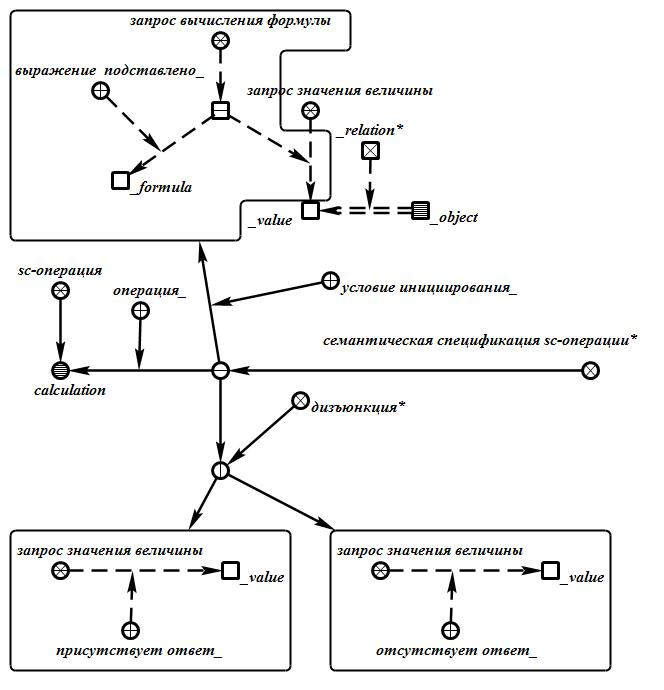
\includegraphics[scale=0.5]{images/part7/chapter_learning_systems/step1.jpg}
	\caption{Семантическая спецификация операции вычисления формулы}
	\label{fig:step1}
\end{figure}

Этап реализации также можно разбить на два шага:

\begin{textitemize}
	\item Разработка алгоритма операции
	\item Реализация программы на подходящем языке. Предпочтительно использовать специально адаптированный язык SCP (semantic code programming).
\end{textitemize}

SCP --- специальный язык программирования, предназначенный для обработки семантических сетей.

Опишем алгоритм работы операции:

\begin{enumerate}
	\item
	Проверяем корректность структуры, которая представляет собой запрос.
	\item
	Из запроса получаем информацию об искомой величине.
	\item
	Находим узел, обозначающий искомую величину в формуле.
	\item
	Находим в формуле все связки отношений ``сложение*'', ``произведение*'' и ``возведение в степень*''.
	\item
	Просматриваем все связки, найденные в шаге 4.
	
	\begin{enumerate}
		\def\labelenumii{\arabic{enumii}.}
		\item
		Если связка принадлежит классу отношения ``сложение*'', то инициируем операцию сложения.
		\item
		Если связка принадлежит классу отношения ``произведение*'', то инициируем операцию умножения.
		\item
		Если связка принадлежит классу отношения ``возведение в степень*'', то инициируем операцию возведения в степень.
		\item
		Если количество выполняемых операций превысило определенный пользователем предел, то генерируем факт отсутствия ответа и завершаем работу операции.
	\end{enumerate}
	\item
	Если значение искомой величины не посчитано, то переходим к шагу 5.
	\item
	Генерируем факт присутствия ответа.
\end{enumerate}

\textbf{Пример протокола решения задачи}

Опишем протокол решения вышеописанной задачи. Протокол отражает последовательность запуска и выполнения операций, текущие условия их запуска, а также результаты выполнения каждой из операций.

\begin{enumerate}
	\item
	В памяти появляется конструкция вида:
\end{enumerate}

\begin{figure}[H]
	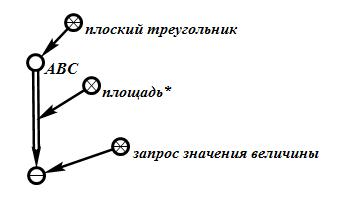
\includegraphics[scale=0.5]{images/part7/chapter_learning_systems/step2.jpg}
	\caption{Запрос значении площади треугольника АВС}
	\label{fig:step2}
\end{figure}

Запускаются операции find\_value и find\_formula, при этом выполнение find\_formula завершается, так как конструкция не полностью соответствует условиям запуска. find\_value проверяет наличие значения указанной величины и, не найдя его, заявляет о его отсутствии:

\begin{figure}[H]
	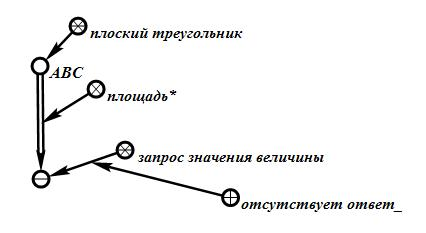
\includegraphics[scale=0.5]{images/part7/chapter_learning_systems/step3.jpg}
	\caption{Результат работы операции find\_value}
	\label{fig:step3}
\end{figure}

\begin{enumerate}
	\setcounter{enumi}{1}
	\item
	Снова запускаются операции find\_value и find\_formula, при этом выполнение find\_value завершается, т.к. конструкция не полностью соответствует условиям запуска.
\end{enumerate}

Операция find\_formula производит поиск в базе знаний подходящей формулы, которая позволила бы вычислить значение требуемой величины у указанного объекта. Под формулой понимается некоторое импликативное логическое высказывание, справедливое для произвольного класса объектов, которому принадлежит рассматриваемый объект (в данном случае --- треугольник), в посылке которого описаны требуемые для вычисления значения, а в заключении --- собственно арифметическое выражение, вычисление которого приводит к получению требуемого результата. В данном случае также используется сокращенная форма высказывания о всеобщности, то есть по умолчанию квантором всеобщности связываются те переменные, которые присутствуют в обеих частях высказывания.

\begin{figure}[H]
	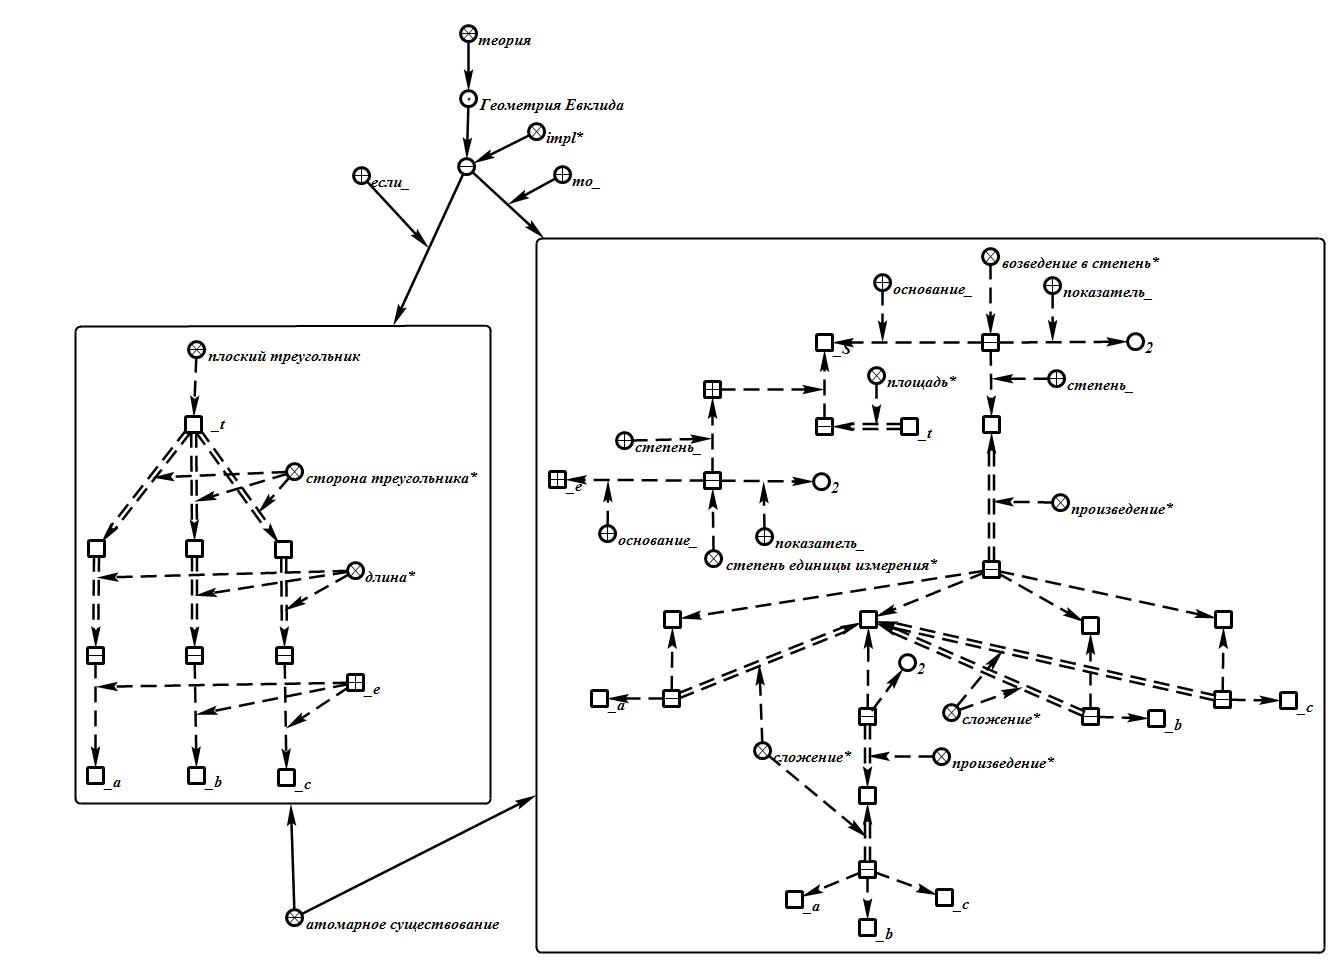
\includegraphics[width=1\linewidth]{images/part7/chapter_learning_systems/step4.jpg}
	\caption{Пример формулы --- формула Герона для вычисления площади треугольника}
	\label{fig:step4}
\end{figure}

При просмотре каждой из формул производится проверка на соответствие предполагаемого результата желаемому и проверка наличия в базе знаний всей необходимой информации. Например, в данном случае проверяется тот факт, что формула Герона позволяет вычислить именно площадь (а не периметр) треугольника (а не четырехугольника или круга). Далее проверяется тот факт, что в базе присутствуют длины всех трех сторон данного треугольника, что позволит воспользоваться именно формулой Герона. В противном случае перебор формул продолжается. В данном случае перебор формул заканчивается на формуле Герона. В памяти генерируется запрос на подстановку конкретных значений в формулу:

\begin{figure}[H]
	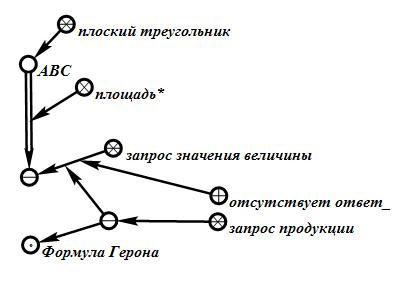
\includegraphics[scale=0.5]{images/part7/chapter_learning_systems/step5.jpg}
	\caption{Запрос на унификацию формулы}
	\label{fig:step5}
\end{figure}

\begin{enumerate}
	\setcounter{enumi}{2}
	\item
	Запускается операция find\_value\_production, задачей которой является унификация предложенной формулы константами из базы знаний. Операция использует посылку формулы для поиска значений, соответствующих именно указанному объекту (в данном случае -- длин треугольника АВС, а не какого-либо другого треугольника). После этого отбираются значения переменных, связанных квантором всеобщности, и производится генерация арифметического выражения с подстановкой в него значений связанных переменных из формулы. Результатом работы является константное арифметическое выражение, требующее вычисления, о чем сообщается путем генерации соответствующей конструкции.
	\item
	Далее запускается операция calculation, алгоритм и условия срабатывания которой подробно рассмотрены выше.
\end{enumerate}

В результате последовательного выполнения указанного набора операций у указанного объекта явно указывается значение требуемого параметра.